\documentclass[12pt]{article}
%\usepackage[utf8]{inputenc}
%\documentclass[UTF8]{ctexart}
%\usepackage[UTF8, heading = false, scheme = plain]{ctex}
\usepackage{geometry}
%geometry{a4paper,scale=0.9}
\geometry{a4paper,left=1cm,right=1cm,top=1cm,bottom=2cm}
\usepackage{amsfonts}
\usepackage{color}
\usepackage{url}
%\usepackage{biblatex}
\usepackage{amsmath}
\usepackage{amssymb}
\usepackage{latexsym}
\usepackage{cite}
%\addbibresource{ref.bib}
%\bibliography{ref.bib}
\usepackage{caption}
\usepackage{graphicx, subfig}
\usepackage{float}
%\usepackage[fontset=ubuntu]{ctex}
%\usepackage{fontspec}
\usepackage{xeCJK}
%\usepackage[colorlinks,
%anchorcolor=black,
%citecolor=black]{hyperref}
%\setmainfont{SimSun}
\usepackage[section]{placeins}
\usepackage{enumitem}
\usepackage{framed}
\usepackage[framemethod=TikZ]{mdframed}
\usepackage{indentfirst}
\usepackage{setspace}%使用间距宏包
\linespread{1.5}
%\title{预备知识}
%\author{leolinuxer }
%\date{June 2020}


\title{线性代数基础知识}
\author{leolinuxer}
%\date{June 2020}

\begin{document}
\maketitle

\section{线性代数解决什么问题\cite{Why_Learn_Linear_Algebra}}
线性代数研究的是\textbf{如何解决线性问题};如何\textbf{把复杂问题线性化}是别的学科的内容,比如《微积分》、《信号与系统》等。

线性代数讨论的线性问题包括:
\begin{itemize}
    \item 向量、向量空间:
    \item \textbf{关于向量、向量空间的函数},也称为矩阵函数;矩阵可以对向量进行变换
    \item 对矩阵函数进行坐标变换
\end{itemize}

举个简单的例子\cite{Cannot_Understand_Linear_Algebra},线性的”东西“(立方体、直线、平面等)可以用向量;矩阵可以对向量进行变换,比如通过旋转矩阵可以让某个正方形变换为旋转后的正方形;行列式代表的是矩阵变换前后的面积(体积)之比;

给定旋转矩阵:
$$
\begin{bmatrix}
\cos(\theta) & -\sin(\theta) \\
\sin(\theta) &  \cos(\theta) 
\end{bmatrix}
$$

很显然旋转正方形不会导致面积改变,所以旋转矩阵变换前后的面积之比为1,或者说行列式为1:
$$
\begin{vmatrix}
\cos(\theta) & -\sin(\theta) \\
\sin(\theta) &  \cos(\theta) 
\end{vmatrix}
 = \cos(\theta)\cos(\theta) + \sin(\theta)\sin(\theta) = 1
 $$

\section{矩阵名称的来源}
\subsection{高斯消元法}
已知线性方程组:
$$
\begin{cases}
1x+2y=3\\
3x+4y=5\\
\end{cases}
$$

从几何上来讲,两个方程都是直线,求解方程组就是找到两根直线的交点;因为都是直线,所以我们称为线性方程组。求解的思路几乎是句废话,即找到交点的$x,y$坐标。也就是把方程化成这个样子:
$$
\begin{cases}
x = ?\\
y = ?\\
\end{cases}
$$

这就是高斯消元法的目标。
\subsection{高斯消元法的思路\cite{From_Gauss_Elimination_To_Matrix_Multiplication}}
要达到这个目标,高斯消元法的思路是,把原线性方程组:
$$
\begin{cases}
a_{11}x + a_{12}y + a_{13}z = d_1 \\
b_{11}x + b_{12}y + b_{13}z = d_2 \\
c_{11}x + c_{12}y + c_{13}z = d_3 \\
\end{cases}
$$

转换为如下形式:
$$
\begin{cases}
a_{11}x + 0y + 0z = d_1' \\
0x + b_{12}y + 0z = d_2' \\
0x + 0y + c_{13}z = d_3' \\
\end{cases}
$$

\subsection{标记法}
英国数学家阿瑟·凯莱(1821-1895)对于看似简单的高斯消元法进行了研究,得出了惊人的结果。他当时研究矩阵的动机出于对线性方程组计算的简化。

对于上面的线性方程组,在固定未知数的顺序($x$出现在第一个位置,$y$出现在第二个位置,常数在等号右边)后,且保证每个未知数都出现(不出现时,系数为0),方程组就只需要系数来表示了。按照上面的规定,方程组可以简写为如下数块:
$$
\begin{pmatrix}
a_{11} & a_{12} & a_{13} & b_{1} \\
a_{21} & a_{22} & a_{23} & b_{2} \\
a_{31} & a_{32} & a_{33} & b_{3} \\
\end{pmatrix}
$$

阿瑟·凯莱在1858年的《矩阵理论纪要》的论文中,给这个数块以合法的数学地位,取了一个名字:\textbf{矩阵}。

\section{理解矩阵\cite{How_To_Understand_Matrix_Multiplication}}
\textcolor{red}{正确的观点是把矩阵看作函数,这样很多疑惑就可以迎刃而解。}

\subsection{矩阵是一个函数}
\subsubsection{直线函数与矩阵}
我们熟悉的直线函数 $ax = y$,把点 $(x,0)$ 映射到 点$(0,ax)$。我们通过矩阵:$A\vec{x} = \vec{y}$ 也可以完成这个映射,令:
$$
A=
\begin{pmatrix}
0&1\\
a&0
\end{pmatrix}
$$

也可以完成:
$$
A\vec{x}=
\begin{pmatrix}
0&1\\
a&0
\end{pmatrix}
\begin{pmatrix}
x\\
0
\end{pmatrix}
=
\begin{pmatrix}
0\\
ax
\end{pmatrix}
$$

\subsubsection{矩阵的优点}
对于:$ax=y,x\in\mathbb{R},y\in\mathbb{R}$ 只能完成实数到实数的映射:
$x\to y\implies \mathbb{R}\to\mathbb{R}$

但是对于:$A\vec{x}=\vec{y},\vec{x}\in\mathbb{R}^n,\vec{y}\in\mathbb{R}^m$可以完成更广泛的映射:
$\vec{x}\to \vec{y}\implies \mathbb{R}^n\to\mathbb{R}^m$

\textbf{为了完成这一点,矩阵$A$就不再是系数$a$了,而是一个函数(或者说是映射)。}

或许写成这样,矩阵乘法看起来更像是函数:$A(\vec{x})=\vec{y}$

假设$\vec{x}$所在平面为$V$,而$\vec{y}$所在平面为$W$,$\vec{x}$通过矩阵$A$映射到了$\vec{y}$,可以如下表示:
\begin{figure}[H]
\centering
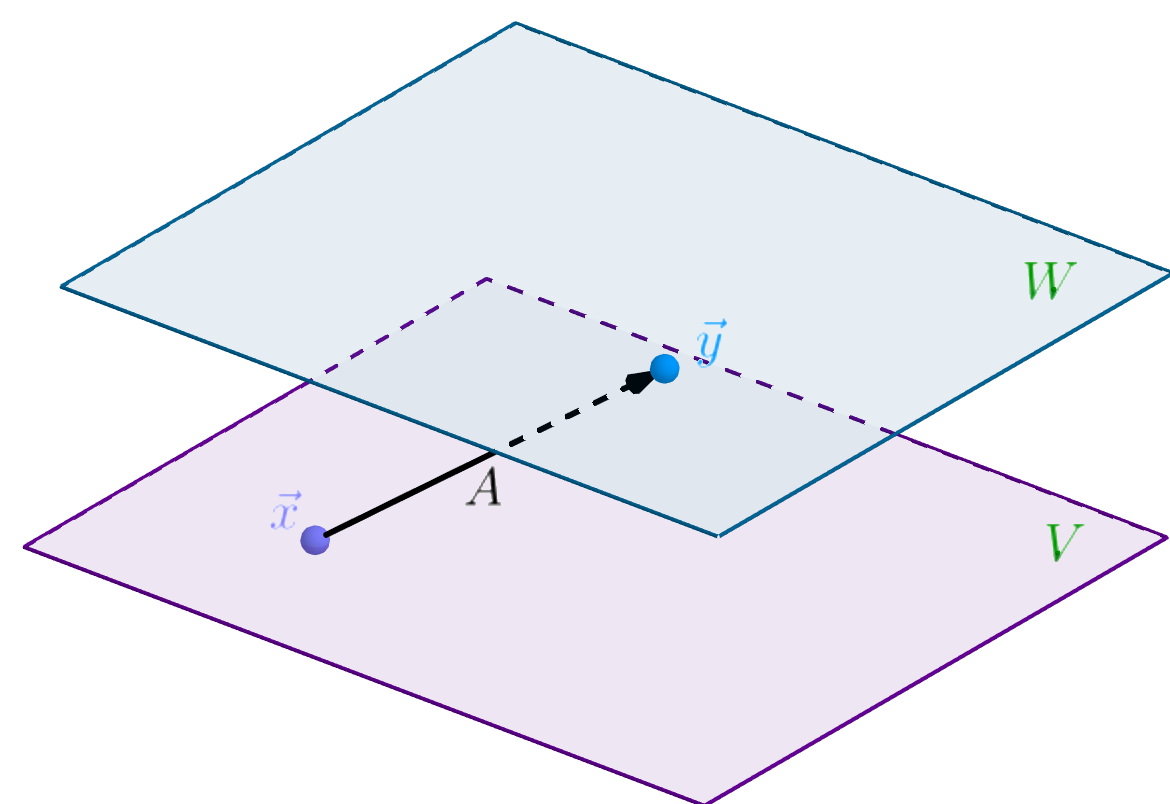
\includegraphics[width=.5\textwidth]{fig/UnderstandMatrixMultiplication_1.png} 
\end{figure}

$A$这个映射的特殊之处是,$V$上的直线通过$A$映射到$W$上也是直线:
\begin{figure}[H]
\centering
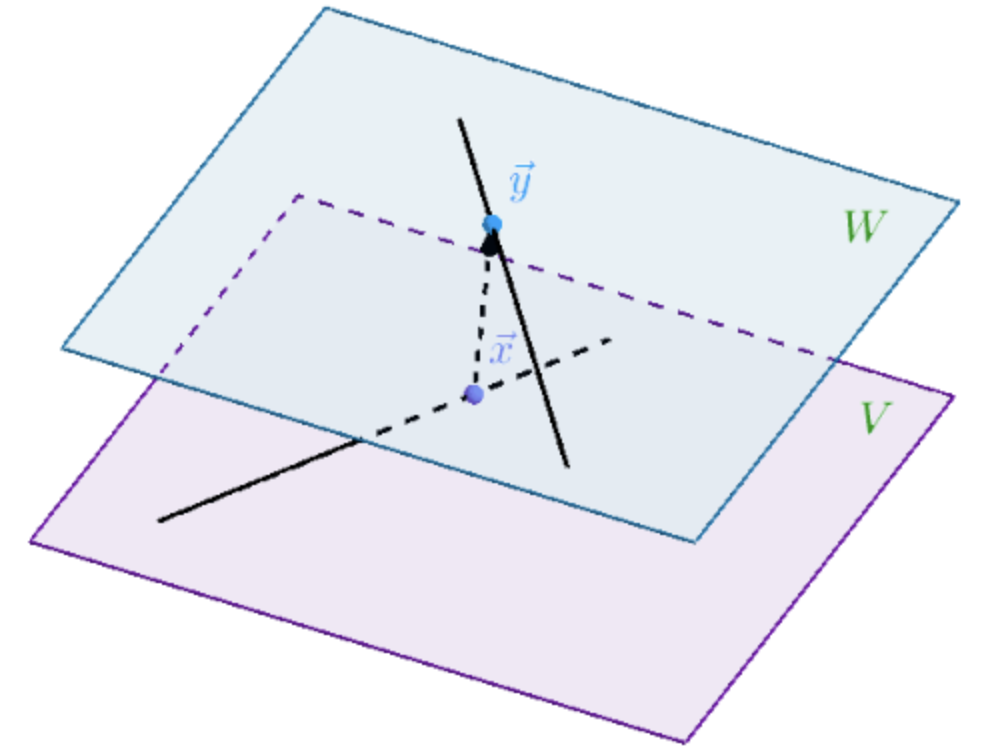
\includegraphics[width=.5\textwidth]{fig/UnderstandMatrixMultiplication_2.png}
\end{figure}

所以矩阵也被称为线性映射。

\subsection{矩阵函数的工作方式}
我们来看看矩阵$A$是如何工作的。
为了方便后面的讲解,把之前表示线性映射的3D图变为2D图:
\begin{figure}[H]
\centering
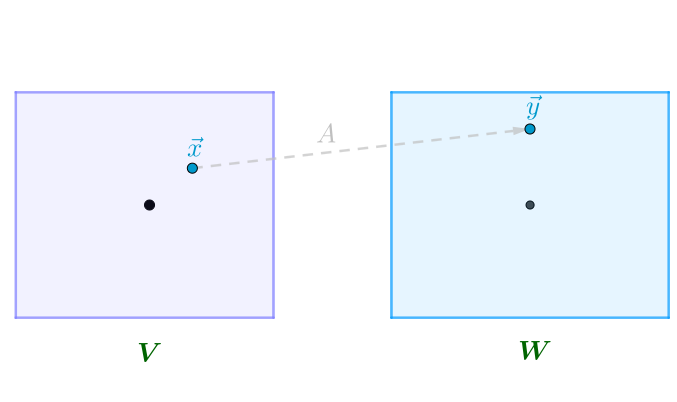
\includegraphics[width=.5\textwidth]{fig/UnderstandMatrixMultiplication_3.png}
\end{figure}

为了画图方便,$\vec{x}$所在平面为$V$、$\vec{y}$所在平面为$W$,都是二维平面,即$\mathbb{R}^2$。

\subsubsection{坐标}
研究线性映射,最重要的是搞清楚当前处在哪个基下。我们先来看看:
$\vec{x}=\begin{pmatrix}x_1\\x_2\end{pmatrix}\qquad\vec{y}=\begin{pmatrix}y_1\\y_2\end{pmatrix}$的基。

$\vec{x},\vec{y}$的基默认为各自向量空间下的自然基,其自然基为(即$\mathbb{R}^2$下的自然基):
$$\vec{i}=\begin{pmatrix}1\\0\end{pmatrix}\qquad\vec{j}=\begin{pmatrix}0\\1\end{pmatrix}$$

所以:
$$\vec{x}=x_1\vec{i}+x_2\vec{j}\qquad\vec{y}=y_1\vec{i}+y_2\vec{j}$$
\begin{figure}[H]
\centering
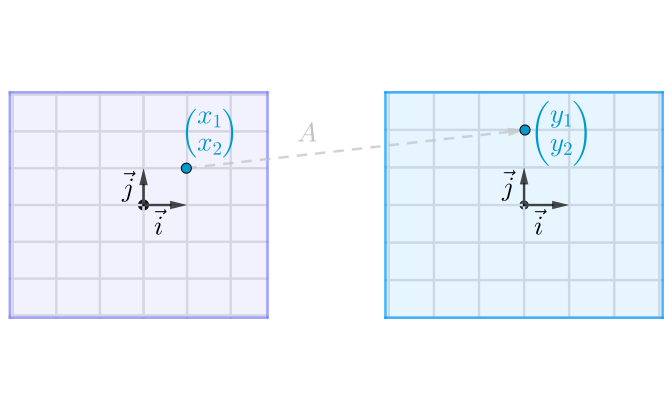
\includegraphics[width=.5\textwidth]{fig/UnderstandMatrixMultiplication_4.png}
\end{figure}

\subsubsection{映射法则的工作原理}
为了说清楚映射法则$A$是怎么工作的,我们把$A$也用一个空间表示,$V$会通过$A$映射到$W$:
\begin{figure}[H]
\centering
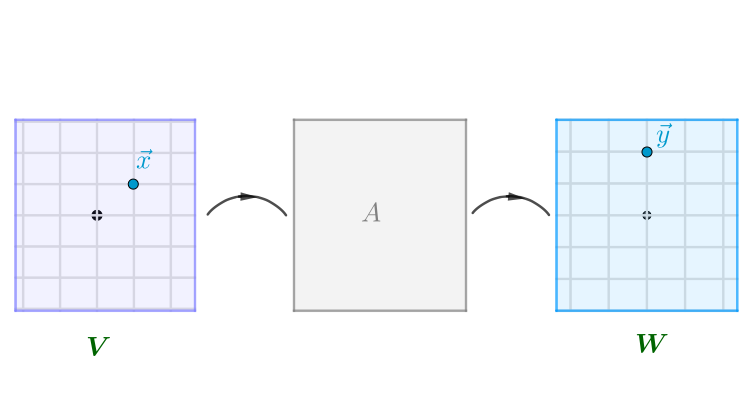
\includegraphics[width=.5\textwidth]{fig/UnderstandMatrixMultiplication_5.png}
\end{figure}

若:$A=\begin{pmatrix}\vec{c_1},&\vec{c_2}\end{pmatrix}$其中$\vec{c_1},\vec{c_2}$为$A$的列向量。
根据矩阵乘法的规则有:
$A\vec{x}=x_1\vec{c_1}+x_2\vec{c_2}$
则$A\vec{x}$相当于在$A$空间中,以$\vec{c_1},\vec{c_2}$为基,坐标为$\begin{pmatrix}x_1\\x_2\end{pmatrix}$的向量:
\begin{figure}[H]
\centering
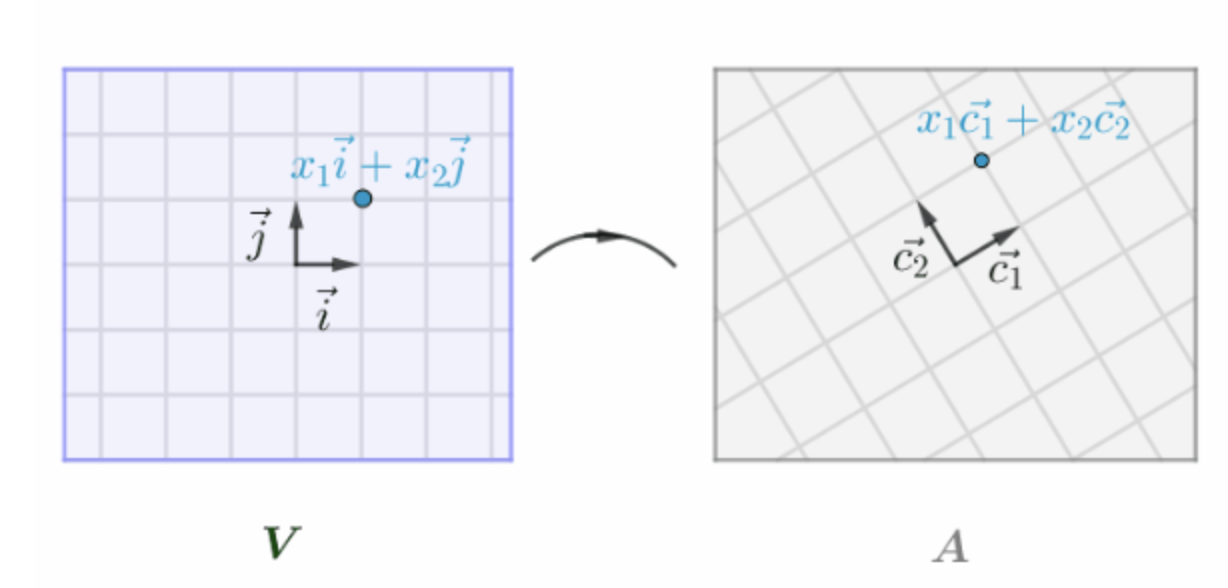
\includegraphics[width=.8\textwidth]{fig/UnderstandMatrixMultiplication_6.png}
\end{figure}

\begin{framed}  
%\verb|\documentstyle[ifthen,12pt,titlepage]{article}|
举例说明 $A\vec{x}=x_1\vec{c_1}+x_2\vec{c_2}$:
$$
A = 
\begin{pmatrix}
\vec{c_1},&\vec{c_2}
\end{pmatrix} = 
\begin{pmatrix}
c_{11},&c_{12} \\
c_{21},&c_{22}
\end{pmatrix} 
$$
$$
A\vec{x} = 
\begin{pmatrix}
c_{11},&c_{12} \\
c_{21},&c_{22}
\end{pmatrix} 
\begin{pmatrix}
x_1 \\
x_2
\end{pmatrix} = 
\begin{pmatrix}
c_{11}x_1,&c_{12}x_2 \\
c_{21}x_1,&c_{22}x_2
\end{pmatrix} = 
x_1\begin{pmatrix}c_{11}\\c_{21}\end{pmatrix} + x_2\begin{pmatrix}c_{12}\\c_{22}\end{pmatrix} = x_1\vec{c_1}+x_2\vec{c_2}
$$
\end{framed}

再将$A\vec{x}$向量用自然基表示:
\begin{figure}[H]
\centering
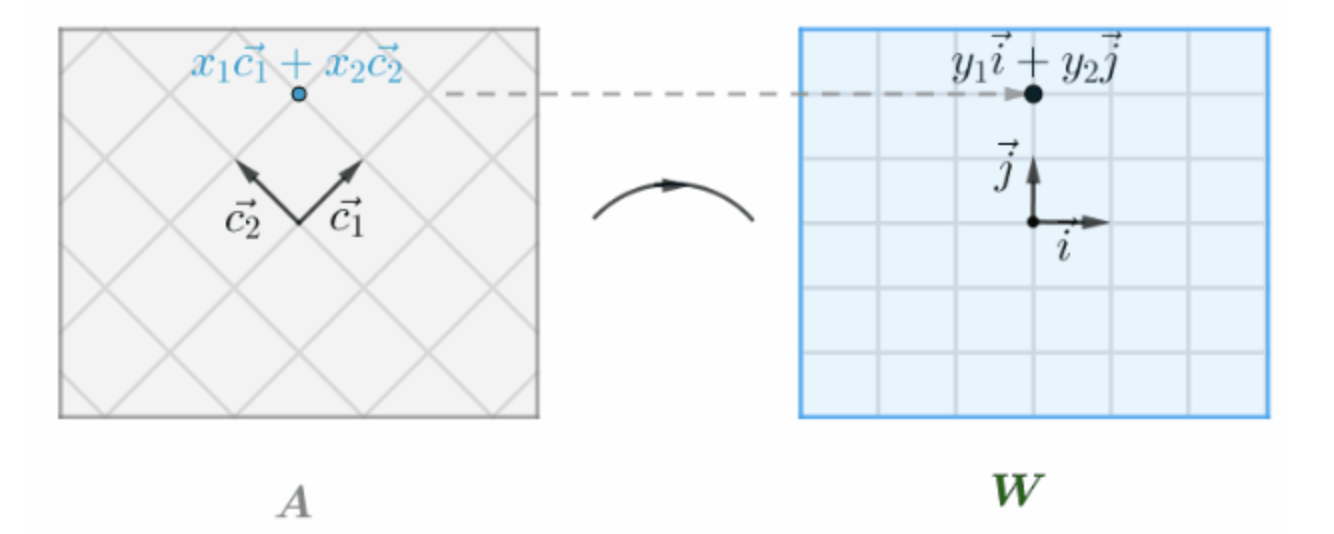
\includegraphics[width=.8\textwidth]{fig/UnderstandMatrixMultiplication_7.png}
\end{figure}

整体来说,就是\textbf{基改变,导致向量的坐标发生变化:}
\begin{figure}[H]
\centering
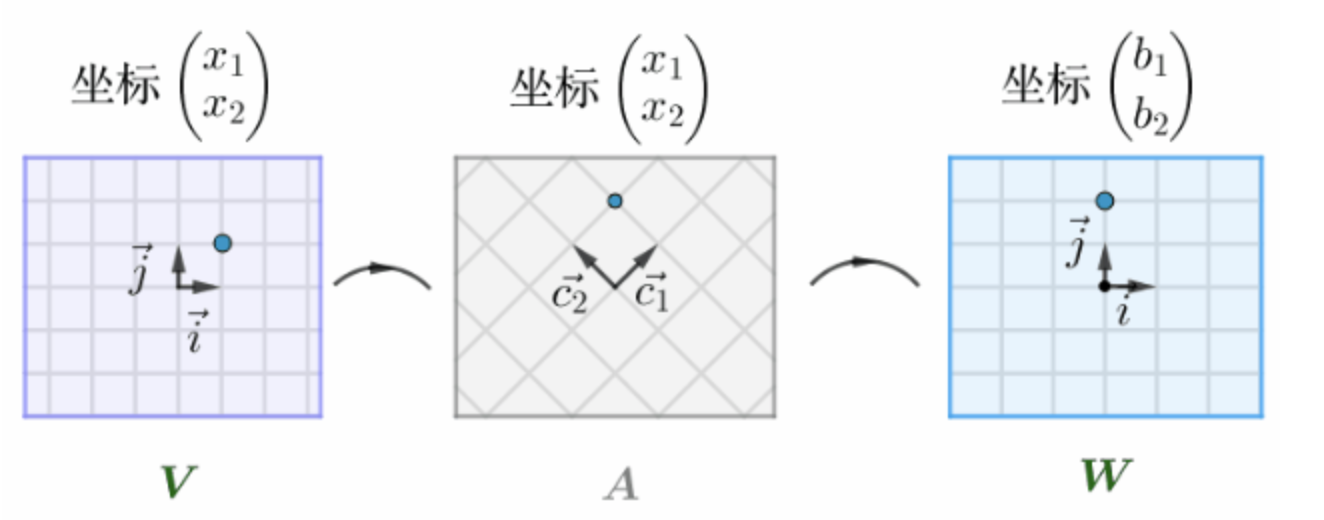
\includegraphics[width=.8\textwidth]{fig/UnderstandMatrixMultiplication_8.png}
\end{figure}

\subsubsection{传送门}
$A$有点像可以穿越空间的传送门,它的传送规则是,根据你进入传送门的时空坐标,把你送到另外一个时空对应的位置。

\subsection{复合函数和乘法交换律}
通过$G$把$\vec{x}$映射到$G(\vec{x})$,再通过$F$把$G(\vec{x})$映射到$\vec{y}$,矩阵的乘法$FG$可以如下图所示:
\begin{figure}[H]
\centering
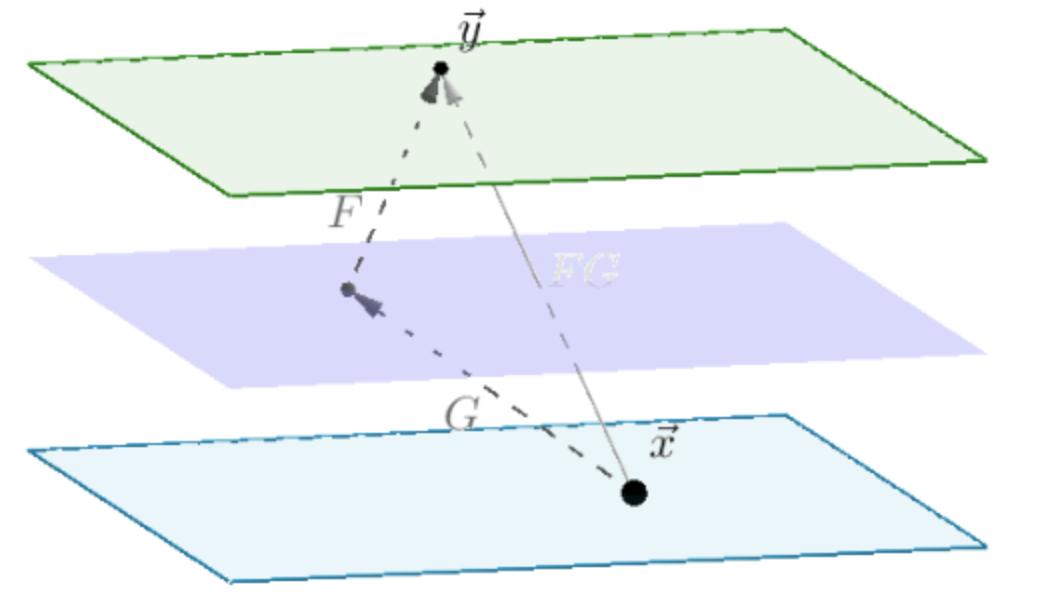
\includegraphics[width=.8\textwidth]{fig/UnderstandMatrixMultiplication_9.png}
\end{figure}

所以\textbf{矩阵乘法 $FG$实际上就是复合函数:
$FG \rightarrow F(G)$}

而函数一般是不满足交换律的,比如:
$f(x)=sin(x)\quad g(x)=x^2$
那么:
$f(g(x))=sin(x^2)\ne g(f(x))=sin^2(x)$
那么矩阵乘法不满足交换律也很好理解了。

\textbf{即从复合函数的角度看(矩阵乘法就是复合函数),矩阵乘法不满足交换律是显然的。}

\section{理解线性变换和仿射变换\cite{How_To_Understand_Affine_Transformation}}
\subsection{线性变换}
线性变换的几何直观有三个要点:
\begin{itemize}
    \item 变换前是直线的,变换后依然是直线
    \item 直线比例保持不变
    \item \textbf{变换前是原点的,变换后依然是原点}
\end{itemize}

比如旋转:对于以原点为中心的正方形,无论怎么旋转,之前的边是直线,之后的边仍然是直线;之前和之后的边长比例保持1:1;之前中心在原点,之后中心仍然在原点;

比如推移:把正方形推移一下(变成平行四边形),直线还是直线;比例还是原来的比例;原点还是原点;

比如旋转加推移,仍然保持上面三个性质不变。

\subsubsection{代数方式描述线性变换}
比如给定一个点$A$,它的坐标为:$(a,b)$;

我们也可以把它看做一个矢量和点以示区别,表示为矩阵:$\vec{A} = \begin{bmatrix}a \\ b\end{bmatrix}$;

用旋转矩阵
$$
T_{rotate}=\begin{bmatrix}cos(\theta)&-sin(\theta)\\sin(\theta)&cos(\theta)\end{bmatrix}
$$

与 $\vec{A}$ 进行矩阵乘法:
$$
T_{rotate}\vec{A} = \vec{A'}
$$

对正方形的每个点都运用 $T_{rotate}$ 就完成了旋转。

总结下来,线性变换是通过矩阵乘法来实现的。

\subsection{仿射变换}
仿射变换从几何直观只有两个要点:
\begin{itemize}
    \item 变换前是直线的,变换后依然是直线
    \item 直线比例保持不变
\end{itemize}

少了原点保持不变这一条。
;
比如允许平移:平移后,直线还是直线,比例还是那个比例,但是原点却发生了变化。

\textbf{因此,平移不再是线性变化了,而是仿射变化。}

\subsubsection{代数方式描述仿射变换}
线性变换是通过矩阵乘法来实现的,仿射变换不能光通过矩阵乘法来实现,还得有加法。

把平移前的中心点称为$O$点,平移后的中心点称为$b$点;令$O$点坐标为 $\vec{x}$,先对 $\vec{x}$ 进行线性变换,$A\vec{x}$,因为是原点,所以任意线性变换都保持不变。

$Ax+b$就可以把$A\vec{x}$移动到 $b$ 点。

所以我们表示仿射变换为:
$$
\vec{y} = A\vec{x} + b
$$

\subsection{通过线性变换来完成仿射变换}
将仿射变换的方程式改写下,可以发现仿射变换和线性变换的关系:
$$
\vec{y} = A\vec{x} + b \Rightarrow 
\begin{bmatrix}
\vec{y}\\
1
\end{bmatrix} = 
\begin{bmatrix}
A & \vec{b}\\
0 & 1
\end{bmatrix}
\begin{bmatrix}
\vec{x}\\
1
\end{bmatrix}
$$

也就是说,\textcolor{red}{增加一个维度后,就可以在高维度通过线性变换来完成低维度的仿射变换。}

举个例子:
\begin{figure}[H]
    \centering
    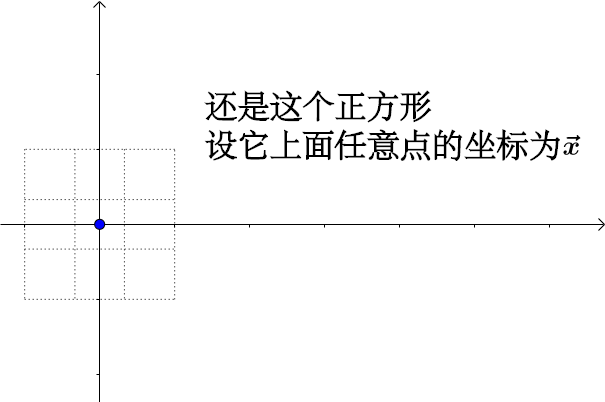
\includegraphics[width=.5\textwidth]{fig/UnderstandAffineTransformation_1.png}
\end{figure}
\begin{figure}[H]
    \centering
    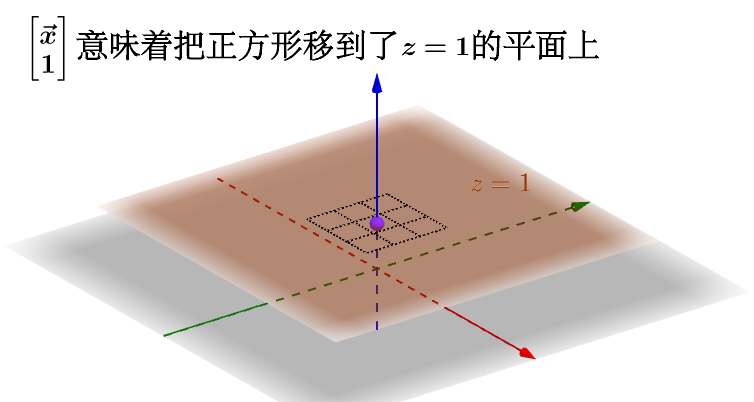
\includegraphics[width=.5\textwidth]{fig/UnderstandAffineTransformation_2.png}
\end{figure}
\begin{figure}[H]
    \centering
    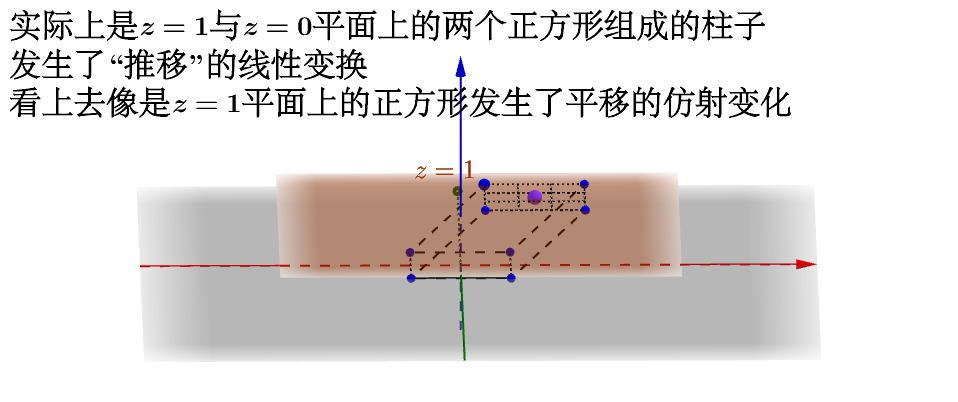
\includegraphics[width=.5\textwidth]{fig/UnderstandAffineTransformation_3.png}
\end{figure}
\begin{figure}[H]
    \centering
    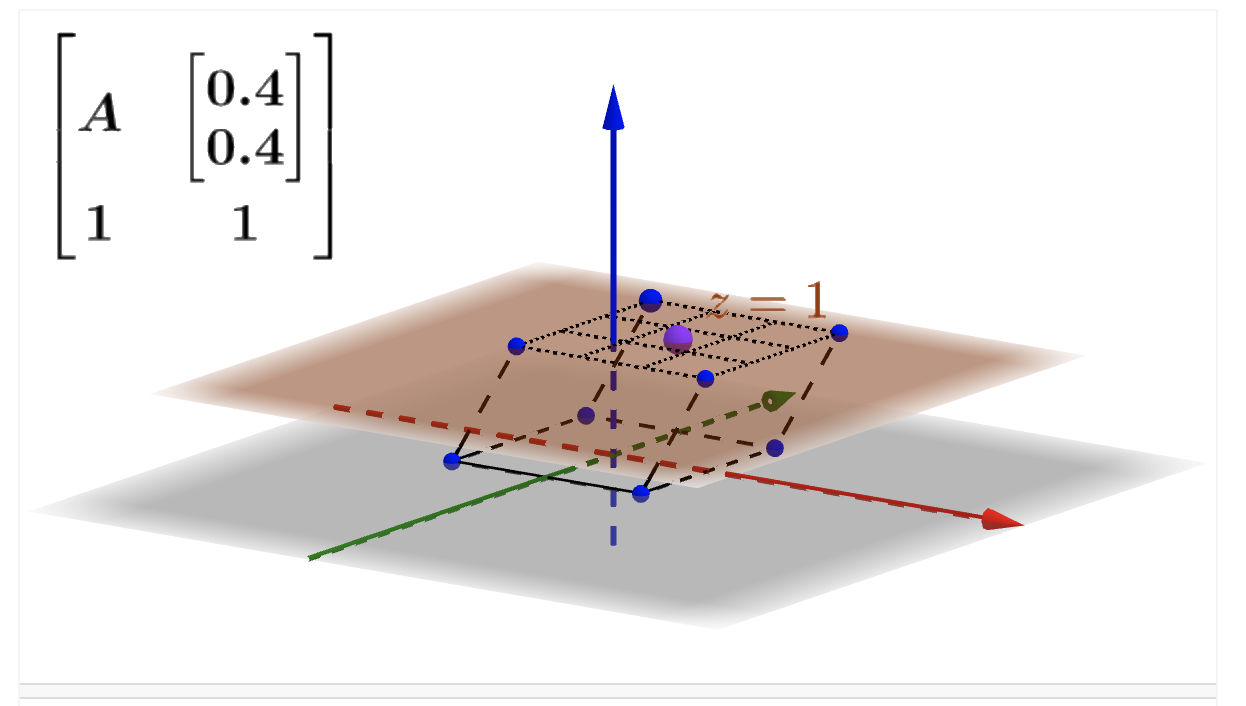
\includegraphics[width=.5\textwidth]{fig/UnderstandAffineTransformation_4.png}
\end{figure}
\begin{figure}[H]
    \centering
    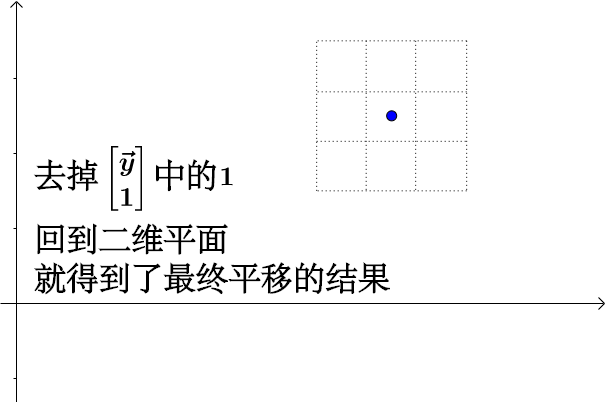
\includegraphics[width=.5\textwidth]{fig/UnderstandAffineTransformation_5.png}
\end{figure}


\section{理解行列式\cite{How_To_Understand_Determinant}}
\subsection{行列式的来历和本质}
人们从解线性方程组开始,最终总结出了行列式。\textbf{行列式的本质是线性变换的伸缩因子。}

\subsection{实现线性变换的矩阵}
比如给定一个点$A$,它的坐标为:$(a,b)$;

我们也可以把它看做一个矢量和点以示区别,表示为矩阵:$\vec{A} = \begin{bmatrix}a \\ b\end{bmatrix}$;

同时,还可以把$\vec{A}$写成$a\vec{i} + b\vec{j}$,其中$\vec{i},\vec{j}$为基向量;

\subsubsection{矩阵变换的其实是基}
举例子来看看,比如旋转(旋转矩阵$T_{rotate}=\begin{bmatrix}cos(\theta)&-sin(\theta)\\sin(\theta)&cos(\theta)\end{bmatrix}$):
$$
T_{rotate}\vec{A} = \vec{A'}
$$

其中 $\vec{A} = a\vec{i} + b\vec{j}$,$\vec{A'} = a\vec{i'} + b\vec{j'}$

所以实际上$T_{rotate}$是\textcolor{red}{改变了基},通过$T_{rotate}$对基进行了变换:$\vec{i} \rightarrow \vec{i'}, \vec{j} \rightarrow \vec{j'}$

如果要说详细点,实际上,\textbf{矩阵的列其实就是变换后的$\vec{i'} \vec{j'}$},这就是矩阵的真正含义。

即对于旋转矩阵:
$$
T_{rotate}=\begin{bmatrix}cos(\theta)&-sin(\theta)\\sin(\theta)&cos(\theta)\end{bmatrix} \quad \Rightarrow \quad 
\vec{i'} = \begin{bmatrix}
cos(\theta) \\ sin(\theta)\end{bmatrix} \quad \vec{j'} = \begin{bmatrix}
\sin(\theta) \\cos(\theta)\end{bmatrix}
$$

我们只需要旋转基,就可以完成正方形的旋转。

\subsection{行列式}
\subsubsection{行列式是线性变换的伸缩因子}
我们还是拿旋转矩阵来举例子:
$$
T_{rotate}=\begin{bmatrix}cos(\theta)&-sin(\theta)\\sin(\theta)&cos(\theta)\end{bmatrix} \Rightarrow |T_{rotate}| = \begin{vmatrix}cos(\theta)&-sin(\theta)\\sin(\theta)&cos(\theta)\end{vmatrix} = \cos^2(\theta) + \sin^2(\theta) = 1
$$

$T_{rotate}$ 的行列式恒等于1,意味着旋转不会改变面积。

同理,对于缩放矩阵:
$$
T_{scale} = \begin{bmatrix}a&0\\0&b\end{bmatrix}
$$
$$
T_{scale}\vec{X} = \begin{bmatrix}a&0\\0&b\end{bmatrix}
\begin{bmatrix}x_1\\x_2\end{bmatrix} = 
x_1\begin{bmatrix}a\\0\end{bmatrix} + 
x_2\begin{bmatrix}0\\b\end{bmatrix}
$$
$$
|T_{scale}| = \begin{vmatrix}a&0\\0&b\end{vmatrix} = ab
$$

变换后,$\vec{i}$对应的坐标会缩放为$a$倍,$\vec{j}$对应的坐标会缩放为$b$倍,面积会缩放为原来的$ab$倍;

掌握了行列式是线性变换的伸缩因子这一点之后,我们就很容易理解各种行列式的值与线性变换的关系。

\subsubsection{行列式大小对变换的影响}
\begin{framed}  
%\verb|\documentstyle[ifthen,12pt,titlepage]{article}|
\textbf{行列式$>0$}
\begin{itemize}
    \item 行列式$>1$,对于图形有放大的作用
    \item 行列式$=1$,图形的大小不会变换
    \item $0<$行列式$<1$,对于图形有缩小的作用
\end{itemize}
\end{framed}

\begin{framed}  
%\verb|\documentstyle[ifthen,12pt,titlepage]{article}|
\textbf{行列式$=0$}

\textbf{行列式等于0,有一个重要的结论是,矩阵不可逆。}

还是以旋转矩阵为例,通过旋转矩阵,逆时针旋转$45^\circ$,旋转矩阵为:
$$
T_{rotate}(45^\circ)=\begin{bmatrix}cos(45^\circ)&-sin(45^\circ)\\sin(45^\circ)&cos(45^\circ)\end{bmatrix}
$$

再通过另外一个旋转矩阵,顺时针旋转$45^\circ$,旋转矩阵为:
$$
T_{rotate}(-45^\circ)=\begin{bmatrix}cos(-45^\circ)&-sin(-45^\circ)\\sin(-45^\circ)&cos(-45^\circ)\end{bmatrix}
$$

两次旋转后,原图形看起来就像没有变换过一样,因此:$T_{rotate}(-45^\circ)$和$T_{rotate}(45^\circ) $ 互为逆矩阵。

有的线性变换是可逆的,有的不行,比如行列式=0这样的线性变换就是不可逆的。从图像上看,图形会缩成一点$\begin{bmatrix}0&0\\0&0\end{bmatrix}$,或者缩成一条直线$\begin{bmatrix}0&0\\0&1\end{bmatrix}$;没有矩阵可以把它们恢复成原来的样子。
\end{framed}

\begin{framed}  
%\verb|\documentstyle[ifthen,12pt,titlepage]{article}|
\textbf{行列式$<0$}

原始图像是这样的:
\begin{figure}[H]
\centering
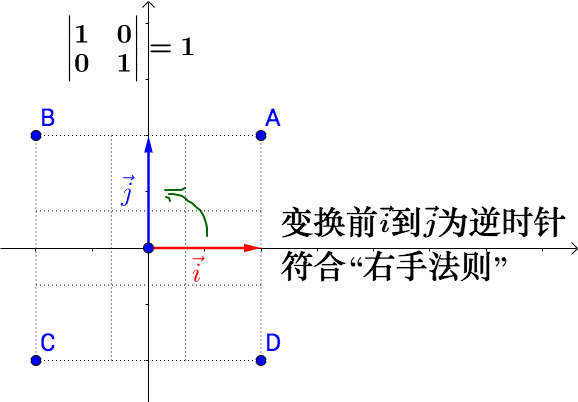
\includegraphics[width=.5\textwidth]{fig/UnderstandDeterminant_1.png}
\end{figure}

被行列式 $< 0$的矩阵线性变换后是这样的:
\begin{figure}[H]
\centering
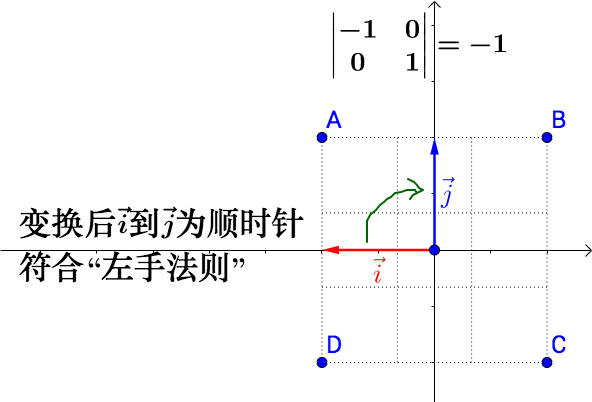
\includegraphics[width=.5\textwidth]{fig/UnderstandDeterminant_2.png}
\end{figure}

行列式 $< 0$其实就是改变了基的“左右手法则”
\end{framed}

\subsection{推论}
知道了行列式的意义,我们就很容易知道,为什么
\begin{itemize}
    \item 矩阵乘法不满足交换律:$T_1T_2 \neq T_2T_1$:因为矩阵乘法相当于复合函数
    \item 但是:$det(T_1T_2) = det(T_2T_1)$:因为面积先缩放为$T_1$倍再缩放为$T_2$倍,与先缩放为$T_2$倍再缩放为$T_1$倍等价
\end{itemize}

同理,可以知道为什么
\begin{itemize}
    \item 二阶矩阵的行列式是\textbf{列}组成的平行四边形的\textbf{面积}(对单位正方形进行了缩放)
\begin{figure}[H]
    \centering
    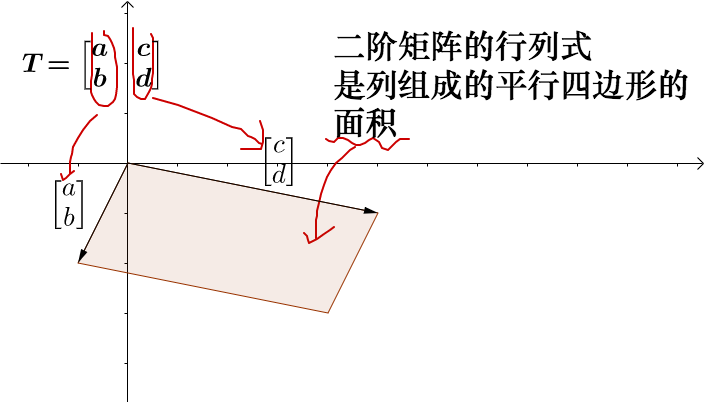
\includegraphics[width=.5\textwidth]{fig/UnderstandDeterminant_3.png}
\end{figure}
\begin{figure}[H]
    \centering
    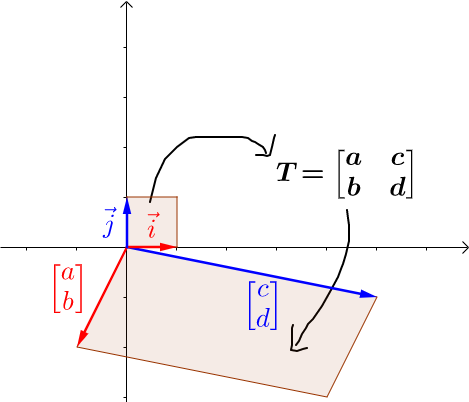
\includegraphics[width=.5\textwidth]{fig/UnderstandDeterminant_4.png}
\end{figure}  
    \item 三阶矩阵的行列式是\textbf{列}组成的平行六面体的\textbf{体积}(对单位正方体进行了缩放
\end{itemize}

\section{理解矩阵的「秩」\cite{How_To_Understand_Rank_Of_Matrix}}
「秩」是图像经过矩阵变换之后的空间维度

「秩」是列空间的维度

\subsection{「秩」是图像经过矩阵变换之后的空间维度}
比如给定原始图像为以原点为中心的正方形,通过旋转矩阵$\begin{bmatrix}cos(\theta)&-sin(\theta)\\sin(\theta)&cos(\theta)\end{bmatrix}$进行变换,变换后的图像是旋转后的正方形(二维);因此,旋转矩阵的「秩」为2。

再通过矩阵$\begin{bmatrix}1&-1\\1&-1\end{bmatrix}$进行变换,变换后的图像是一根一维的直线;因此,该变换矩阵的「秩」为1。

再通过矩阵$\begin{bmatrix}0&0\\0&0\end{bmatrix}$进行变换,变换后的图像是一个零维的点;因此,该变换矩阵的「秩」为0。

\subsection{「秩」是列空间的维度}
\subsubsection{列空间}
我们通过旋转矩阵来解释什么是列空间;给定旋转矩阵
$$
T_{rotate}=
\begin{bmatrix}
    cos(\theta) & -sin(\theta)\\
    sin(\theta) & cos(\theta)
\end{bmatrix}
$$

该旋转矩阵的列向量分别是$\vec{i}=\begin{bmatrix}cos(\theta)\\sin(\theta)\end{bmatrix}$和$\vec{j}=\begin{bmatrix}-sin(\theta)\\cos(\theta)\end{bmatrix}$这两个向量不在一条直线上,我们称其为线性无关。

通过改变$a,b$的值,可以用$a\vec{i} + b\vec{j}$来表示二维平面上的所有点。

所以,\textbf{列空间就是矩阵的列向量所能张成(即通过$a\vec{i} + b\vec{j}$来表示)的空间。}

\textbf{列空间的维度就是「秩」};旋转矩阵的列空间是二维的,所以「秩」就为2。

\subsubsection{矩阵的变换目标是列空间}
给定矢量$\vec{A} = \begin{bmatrix}a\\b\end{bmatrix}$;

同时,矢量$\vec{A} = \begin{bmatrix}a\\b\end{bmatrix}$也可以表示为$a\vec{i}+b\vec{j}$,其中$\vec{i} \vec{j}$ 为基向量。用基来表示的原因是因为矩阵变换的其实是基。

举例子来看看,比如给定旋转矩阵 $T_{rotate}=\begin{bmatrix}cos(\theta)&-sin(\theta)\\sin(\theta)&cos(\theta)\end{bmatrix}$ 作用在矢量 $\vec(A)$上,有:
$$
\vec{A'} = T_{rotate}\vec{A}
$$

其中,$\vec{A} = a\vec{i} + b\vec{j}$,$\vec{A'} = a\vec{i'} + b\vec{j'}$

所以实际上是$T_{rotate}$是\textcolor{red}{改变了基},通过 $T_{rotate}$把$\vec{i} \rightarrow \vec{i'}$,$\vec{j} \rightarrow \vec{j'}$。

如果要说详细点,实际上矩阵的列就是变换后的$\vec{i'} \vec{j'}$,这就是矩阵的真正含义。

所以:$\vec{A} = a\vec{i} + b\vec{j} \Rightarrow \vec{A'} = a\vec{i'} + b\vec{j'}$ 实际上是变换到了$T_{rotate}$的列空间。

\subsubsection{两种定义方式的联系}
用旋转矩阵对二维的正方形进行线性变换,实际上是一个二维空间到另外一个二维空间的变换:

比如对于旋转矩阵,图像从$\vec{i}$,$\vec{j}$张成的空间,变换到$\vec{i'}$,$\vec{j'}$张成的空间。因为都是二维,所以图像维度不变。

但是对于矩阵$\begin{bmatrix}1&-1\\1&-1\end{bmatrix}$他的列空间是一维的;因此,这个矩阵的「秩」就是1,用它对二维的正方形进行线性变换,实际上是一个二维空间到另外一个一维空间的变换(即二维正方形会被压缩到一维直线上);

同理,矩阵$\begin{bmatrix}0&0\\0&0\end{bmatrix}$他的列空间是一个点,所以它的「秩」就是0。

\subsection{关于严格性的一个问题}
上面说矩阵的「秩」是列空间的维度,这并非完全正确的。

列空间的维度准确来说,是「列秩」,行空间的维度是「行秩」,但是,还好有,「秩」=「列秩」=「行秩」是恒成立的。所以直接把「列秩」称为「秩」也不算错误。

\subsection{推论}
了解了秩,就很容易回答下面的问题。

我们知道矩阵是做线性变换的,比如说一个$3\times2$的矩阵,
\begin{figure}[H]
    \centering
    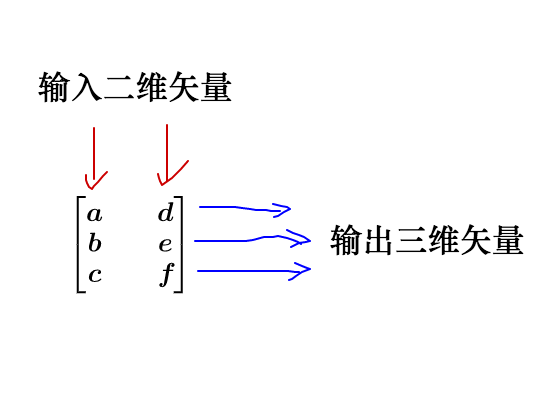
\includegraphics[width=.5\textwidth]{fig/UnderstandDeterminant_5.png}
\end{figure}  

从图像上看,平面上的一个矢量被一个$3\times2$的矩阵变换到了三维空间:
\begin{figure}[H]
    \centering
    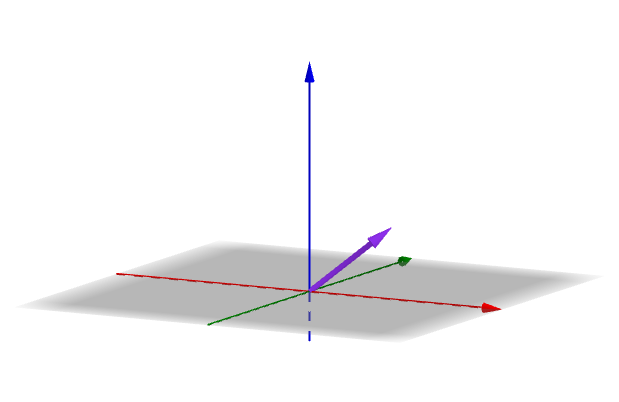
\includegraphics[width=.5\textwidth]{fig/UnderstandDeterminant_6.png}
\end{figure} 

那么,通过$3\times2$的矩阵能否把一个二维正方形变换为一个三维正方体呢?

\section{理解行秩和列秩的关系\cite{Why_Rank_Of_Row_Column_Equal}}
TBD

\section{理解相似矩阵\cite{How_To_Understand_Similar_Matrix}}
相似矩阵的定义是:
设$A,B$都是$n$阶矩阵,若有可逆矩阵$P$,使:
$$
P^{-1}AP=B
$$
则称$B$是$A$的相似矩阵,或说$A$和$B$相似。

\subsection{通俗解释}
观看同样一部电影,坐在不同的位置,各自眼中看到的电影因为位置不同而有所不同(比如清晰度、角度),所以说,“第一排看到的电影”和“最后一排看到的电影”是“相似”的。

那么相似矩阵走进的电影院,放映的是哪部电影?也就是说,什么是不变的呢?是线性变换。

\subsection{坐标转换}
从数学角度上看,相似变换就是进行了坐标转换。

坐标转换是数学中的常用伎俩,目的是简化运算。比如常见的,把直角坐标系($xy$坐标系)的圆方程换元为极坐标($\rho\theta$坐标系)下:
$$
x^2 + y^2 = a^2 \Rightarrow \begin{cases}
\rho = a \\
\theta \in \mathbb{R}
\end{cases}
$$

图像也从左边变为了右边:
\begin{figure}[H]
    \centering
    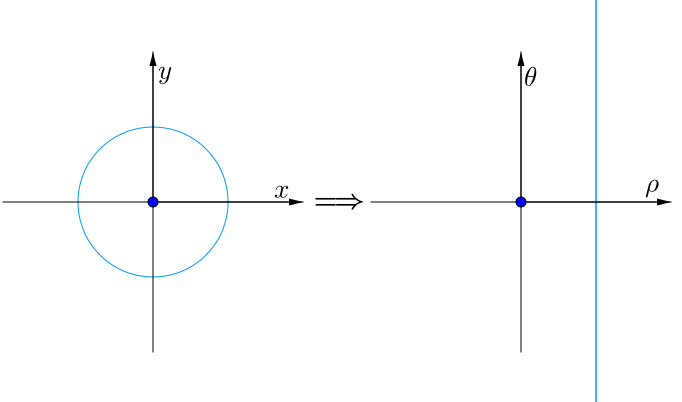
\includegraphics[width=.8\textwidth]{fig/UnderstandSimilarMatrix_1.png}
\end{figure} 

换元之后的代数式和图像都变简单了。相似变换也是这样的目的。

\subsection{线性变换}
\subsubsection{线性函数}
函数我们很早就接触了,直观地讲,就是把$x$轴上的点映射到曲线上。比如函数函数$y=sin(x)$,把$x$轴上的点映射到了正弦曲线上);还有的函数,比如$y=x$,是把$x$轴上的点映射到直线上,我们称为线性函数;

\subsubsection{从线性函数到线性变换}
线性函数其实就是线性变换,为了看起来更像是线性变换,我换一种标记法。

比如之前的$y=x$,我们可以认为是把$(a,0)$点映射到$(0,a)$点,我们称为线性变换$T$,记作:
$$
T:(a,0) \rightarrow (0,a), a \in \mathbb{R}, b \in \mathbb{R}
$$

矩阵的形式很显然如下:
$$
\begin{pmatrix}
0 \\ a
\end{pmatrix}
= \begin{pmatrix}
0 & 1 \\
1 & 0 \\
\end{pmatrix}
\begin{pmatrix}
a \\ 0
\end{pmatrix}
$$

这样做最直接的好处是,\textbf{我们可以轻易的摆脱$x$轴的限制。}

\textbf{只要替换$(a,0)$为平面内所有的点$(a,b)$,我们就可以对整个平面做变换},该线性变换记作:
$$
T:(a,b) \rightarrow (b,a)
$$

进而可以写作矩阵的形式:
$$
\begin{pmatrix}
a \\ b
\end{pmatrix}
= \begin{pmatrix}
0 & 1 \\
1 & 0 \\
\end{pmatrix}
\begin{pmatrix}
a \\ b
\end{pmatrix}
$$

也就是说整个平面的点都可以被变换。

使用线性代数的记号,有:
$$
\vec{x} = \begin{pmatrix}
a \\ b
\end{pmatrix} \quad
\vec{y} = \begin{pmatrix}
b \\ a
\end{pmatrix} \quad
A = \begin{pmatrix}
1&0 \\ 0&1
\end{pmatrix}
$$

即:
$$
\vec{y} = A\vec{x}
$$

进一步,既然$\vec{x},\vec{y}$都是平面上的点,我们可以认为:
\begin{center}
\textbf{线性变换通过矩阵$A$来表示}
\end{center}

而$y=x$只不过是这个 $A$ 的一种特殊情况。

\subsubsection{矩阵$A$与基}
因为 $y=x$ 是基于直角坐标系的,通过这个转换:
$$
y = x \rightarrow A = \begin{pmatrix}
1&0 \\ 0&1
\end{pmatrix}
$$

得到的$A$也是基于直角坐标系的。只是在线性变换中,我们不称为直角坐标系,我们叫做\textbf{标准正交基}。

标准正交基是:
$$
\vec{i} = \begin{pmatrix}1\\0\end{pmatrix}, \vec{j} = \begin{pmatrix}0\\1\end{pmatrix}
$$

它们所张成的线性空间如下:
\begin{figure}[H]
\centering
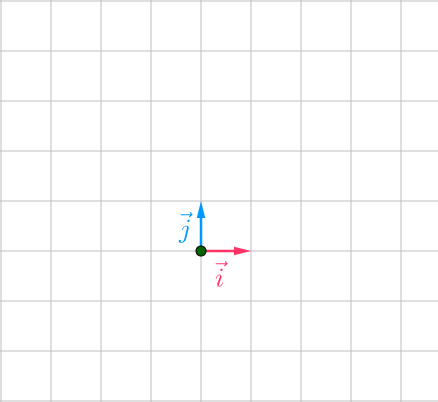
\includegraphics[width=.5\textwidth]{fig/UnderstandSimilarMatrix_2.png} 
\end{figure}

$A$在此基下,完成了镜面反转这个线性变换。

因此,让我们补完之前的结论:
\begin{center}
\textbf{线性变换通过}\textcolor{red}{指定基下的}{矩阵}A\textbf{来表示}
\end{center}

\subsection{相似矩阵}
回到开头给出看电影的例子,同一部“电影”,不同基“看到”的就是不同的矩阵:

\begin{center}
\textbf{同一个线性变换,}\textcolor{red}{不同基下的}\textbf{矩阵,称为相似矩阵}
\end{center}

那怎么得到不同基下的矩阵呢?让我们来看看变换的细节。

\subsubsection{变换的细节}
先上一张图,说明不同基下的矩阵的变换思路,这个图有点复杂,请参照之后的解释一起来看:
\begin{figure}[H]
    \centering
    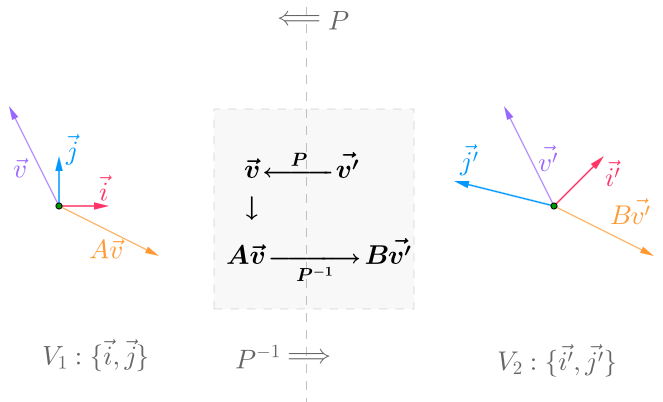
\includegraphics[width=.8\textwidth]{fig/UnderstandSimilarMatrix_3.png}
\end{figure} 

下面是对图的解释:
\begin{itemize}
    \item 有两个基:$V_1:\{\vec{i},\vec{j}\}$和$V_2:\{\vec{i'}, \vec{j}\}$
    \item $V_1 \rightarrow V_2$,可以通过 $P^{-1}$ 转换
    \item $V_2 \rightarrow V_1$,可以通过$P$ 转换
\end{itemize}

整个转换的核心,就是上图正中的文字,解释下:
\begin{itemize}
    \item $\vec{v'}$ 是$V_2$下的点
    \item $\vec{v'}$ 通过 $P$ 变换为 $V_1$ 下的点,即$P\vec{v'}$
    \item 在 $V_1$ 下,通过矩阵 $A$ 完成线性变换,即$AP\vec{v'}$
    \item 通过 $P^{-1}$ 重新变回$V_2$下的点,即$P^{-1}AP\vec{v'}$
\end{itemize}

综上,我们可以有:
$$
B\vec{v'} = P^{-1}AP\vec{v'}
$$

那么$B$和$A$互为相似矩阵。

\textcolor{red}{注意[待验证,应该没问题],这里的 $P$ 只进行了坐标基之间的变换,\textbf{所以$det(P) = \pm 1$};但是 $A$ 是线性变换,\textbf{所以可以有$det(A) \ne \pm 1$}。}


\subsubsection{转换矩阵$P$的计算方法}
给定空间中的点 $m$,它在基 $\vec{i'},\vec{j'}$ 下的坐标$\vec{v'}$可以表示为:
$$
\vec{v'} = \begin{pmatrix}a\\b\end{pmatrix} = a\vec{i'} + b\vec{j'}
$$

如果我们知道了$\vec{i'},\vec{j'}$在$\vec{i},\vec{j}$下的坐标:
$$
\vec{i'} = c\vec{i} + d\vec{j}, \vec{j'} = e\vec{i} + f\vec{j}
$$

那么有:
\begin{align*}
\vec{v'} &= a\vec{i'} + b\vec{j'} \\
    &= a(c\vec{i} + d\vec{j}) + b(e\vec{i} + f\vec{j})
\end{align*}

此时,实际上$m$点的坐标,已经变到了$\vec{i},\vec{j}$下的 $\vec{v}$:
\begin{align*}
\vec{v} &= a(c\vec{i} + d\vec{j}) + b(e\vec{i} + f\vec{j}) \\
    &= (ac+be)\vec{i} + (ad+bf)\vec{j} \\
    &= \begin{pmatrix}c&e\\d&f\end{pmatrix}\begin{pmatrix}a\\b\end{pmatrix} \\
    &= \begin{pmatrix}\vec{i'}&\vec{j'}\end{pmatrix}\vec{v'} \\
    &= P\vec{v'}
\end{align*}

所以$P$其实就是:
$$
P = (\vec{i}, \vec{j})
$$

这里的$\vec{i'},\vec{j'}$是在$\vec{i},\vec{j}$下的坐标。

\subsubsection{对角矩阵}
那么为什么我们需要相似矩阵呢?

比如这个矩阵$A$:
$$
A = \begin{pmatrix}2&-1\\-1&2\end{pmatrix}
$$

可以这样分解:
$$
B = P^{-1}AP = \begin{pmatrix}3&0\\0&1\end{pmatrix}
$$

其中 $P = P^{-1} = \begin{pmatrix}
-\frac{\sqrt{2}}{2}&\frac{\sqrt{2}}{2}\\
\frac{\sqrt{2}}{2}&\frac{\sqrt{2}}{2}
\end{pmatrix}$

$B$就是对角矩阵,看上去就很清爽,所以说相似变换就是坐标转换,转换到一个更方便计算的简单坐标系。

\section{理解二次型\cite{How_To_Understand_Quadratic_Form}}
二次型就是通过矩阵研究二次函数。

通过矩阵来研究二次函数(方程),这就是线性代数中二次型的重点。

\subsection{二次函数(方程)的特点}
最简单的一元二次函数就是:$y = x^2$,给它增加一次项和常数项:$y = x^2 + px + q$ 不会改变它的形状(只会改变对称轴的位置和在 $y$ 轴的截距)

再看二元二次方程:$x^2 + xy + y^2 = 1$
\begin{figure}[H]
    \centering
    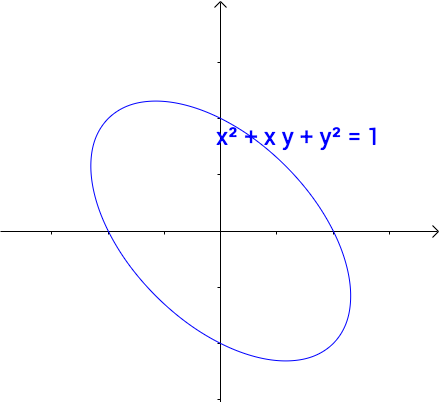
\includegraphics[width=.8\textwidth]{fig/UnderstandQuadraticForm_1.png}
\end{figure} 

给它增加一次项也不会改变形状$x^2 + xy + y^2 + 0.3x = 1$,只是看上去有些伸缩:
\begin{figure}[H]
    \centering
    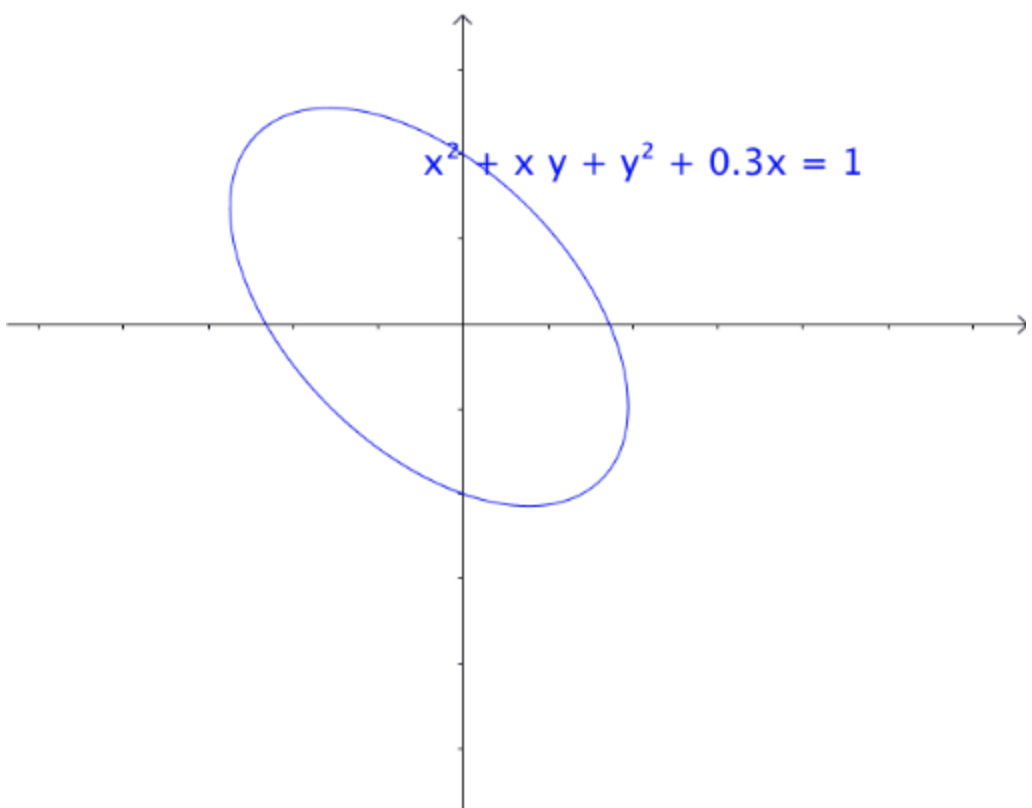
\includegraphics[width=.8\textwidth]{fig/UnderstandQuadraticForm_2.png}
\end{figure} 

所以,对于二次函数或者二次方程,\textbf{二次部分是主要部分,往往研究二次这部分就够了}。

\subsection{通过矩阵来研究二次方程}
因为二次函数(方程)的二次部分最重要,为了方便研究,我们把含有$n$个变量的二次齐次函数:
\begin{align*}
f(x_1, x_2, \cdots, x_n) &= a_{11}x_1^2 + a_{22}x_2^2 + \cdots + a_{nn}x_n^2 \\
 &+ 2a_{12}x_1x_2 + 2a_{13}x_1x_3 + \cdots + 2a_{n-1,n}x_{n-1}x
\end{align*}
或者二次齐次方程称为二次型。

\subsubsection{二次型矩阵}
实际上我们可以通过矩阵来表示二次型:
$$
x^2 - xy + y^2 = 1 \Rightarrow 
\begin{bmatrix}x & y\end{bmatrix}
\begin{bmatrix}1&-0.5\\-0.5&1\end{bmatrix}
\begin{bmatrix}x \\ y\end{bmatrix} = 1
$$

其中,$\left[\begin{smallmatrix}1&-0.5\\-0.5&1\end{smallmatrix}\right]$就是二次型。

更一般的:
$$
ax^2 + 2bxy + cy^2 = 1\Rightarrow 
\begin{bmatrix}x & y\end{bmatrix}
\textcolor{red}{\begin{bmatrix}a&b\\b&c\end{bmatrix}}
\begin{bmatrix}x \\ y\end{bmatrix} = 1
$$

可以写成更线代的形式:
$$
\left.
\begin{matrix}
\begin{bmatrix}x & y\end{bmatrix}
\begin{bmatrix}a&b\\b&c\end{bmatrix}
\begin{bmatrix}x \\ y\end{bmatrix} = 1 \\
\\
X =  \begin{bmatrix}x \\ y\end{bmatrix}\\
\\
A = \begin{bmatrix}a&b\\c&d\end{bmatrix} \\
\end{matrix}
\right\}
\Rightarrow X^TAX
$$

所以有下面一一对应的关系:
\begin{center}
\textbf{对称矩阵$\Longleftrightarrow$二次型矩阵$\Longleftrightarrow$二次型矩阵}
\end{center}

在线代里面,就是通过一个对称矩阵,去研究某个二次型。

\subsubsection{通过矩阵来研究有什么好处}
\textbf{圆锥曲线}

我们来看下,这是一个圆:
\begin{figure}[H]
    \centering
    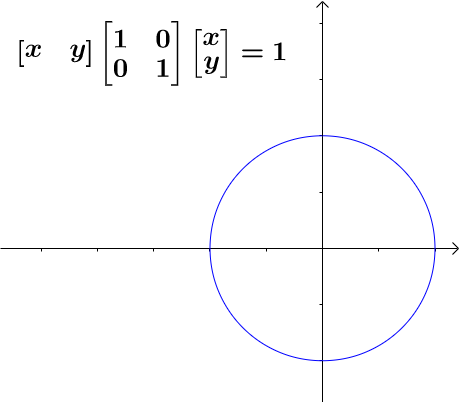
\includegraphics[width=.5\textwidth]{fig/UnderstandQuadraticForm_3.png}
\end{figure} 

然后看改变一下二次型矩阵:
\begin{figure}[H]
    \centering
    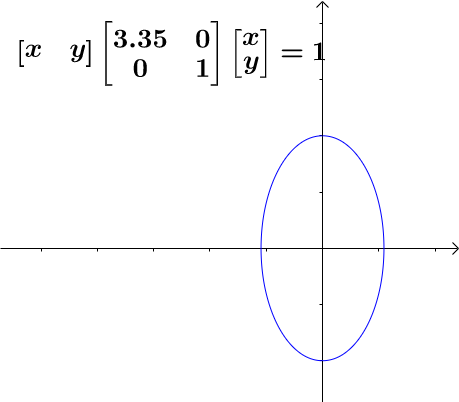
\includegraphics[width=.5\textwidth]{fig/UnderstandQuadraticForm_4.png}
\end{figure} 

所以原来椭圆和圆之间是线性关系(通过矩阵变换就可以从圆变为椭圆)。

继续:
\begin{figure}[H]
    \centering
    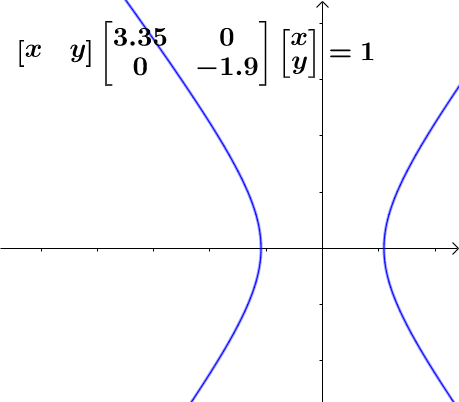
\includegraphics[width=.5\textwidth]{fig/UnderstandQuadraticForm_5.png}
\end{figure} 
双曲线和圆之间也是线性关系(准确的说是仿射的)。其实圆、椭圆、双曲线之间关系很紧密的,统称为圆锥曲线,都是圆锥体和平面的交线。一个平面在圆锥体上运动,可以得到圆、椭圆、双曲线,这也是它们之间具有线性关系的来源(平面的运动是线性的、或者是仿射的)。

\textbf{规范化}

再改变下矩阵:
\begin{figure}[H]
    \centering
    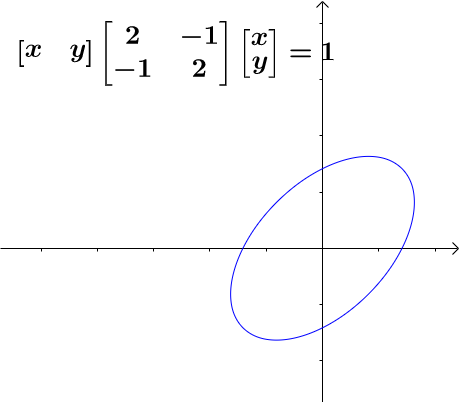
\includegraphics[width=.5\textwidth]{fig/UnderstandQuadraticForm_6.png}
\end{figure} 

这个椭圆看起来有点歪,不太好处理,我们来把它扶正,这就叫做\textbf{规范化}。如果我们对矩阵有更深刻的认识,那么要把它扶正很简单。

首先,矩阵代表了运动,包含:
\begin{itemize}
    \item 旋转
    \item 拉伸
    \item 投影
\end{itemize}

对于方阵,因为没有维度的改变,所以就没有投影这个运动了,只有
\begin{itemize}
    \item 旋转
    \item 拉伸
\end{itemize}

具体到上面的矩阵:
\begin{figure}[H]
    \centering
    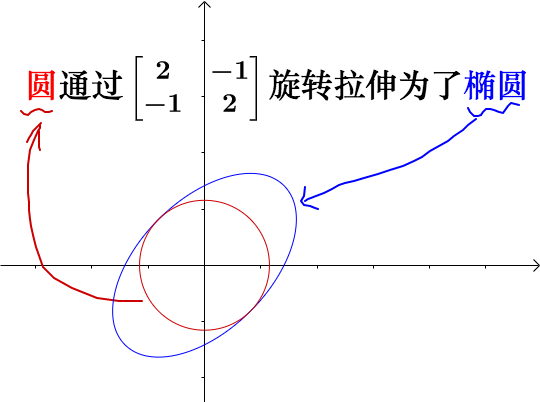
\includegraphics[width=.5\textwidth]{fig/UnderstandQuadraticForm_7.png}
\end{figure} 

我把这个矩阵进行特征值分解:
\begin{figure}[H]
    \centering
    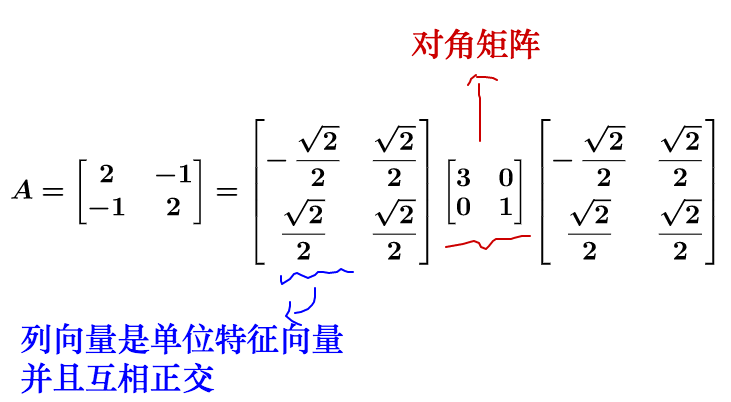
\includegraphics[width=.8\textwidth]{fig/UnderstandQuadraticForm_8.png}
\end{figure} 

对于二次型矩阵,都是对称矩阵,所以特征值分解总可以得到正交矩阵与对角矩阵。特征值分解实际上就是把运动分解了:
\begin{figure}[H]
    \centering
    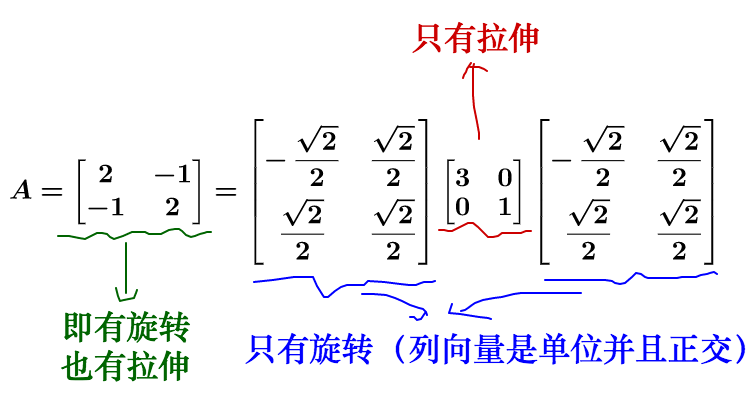
\includegraphics[width=.8\textwidth]{fig/UnderstandQuadraticForm_9.png}
\end{figure} 

那么我们只需要保留拉伸部分,就相当于把矩阵扶正(图中把各自图形的二次型矩阵标注出来了):
\begin{figure}[H]
    \centering
    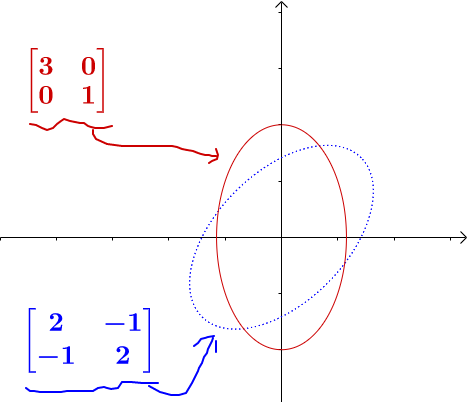
\includegraphics[width=.5\textwidth]{fig/UnderstandQuadraticForm_10.png}
\end{figure} 

所以,用二次型矩阵进行规范化是非常轻松的事情。

\textbf{正定}

正定是对二次函数有效的一个定义,对方程无效。对于二次型函数,$f(x)=x^TAx$:
\begin{itemize}
    \item $f(x)>0, x \ne 0, x \in \mathbb{R}$,则 $f$ 为正定二次型,$A$为正定矩阵
    \item $f(x) \ge 0, x \ne 0, x \in \mathbb{R}$,则 $f$ 为半正定二次型,$A$为半正定矩阵
    \item $f(x) < 0, x \ne 0, x \in \mathbb{R}$,则 $f$ 为负定二次型,$A$为负定矩阵
    \item $f(x) \le 0, x \ne 0, x \in \mathbb{R}$,则 $f$ 为半负定二次型,$A$为半负定矩阵
    \item 以上皆不是,就叫做不定
\end{itemize}

从图像上看,这是正定:
\begin{figure}[H]
    \centering
    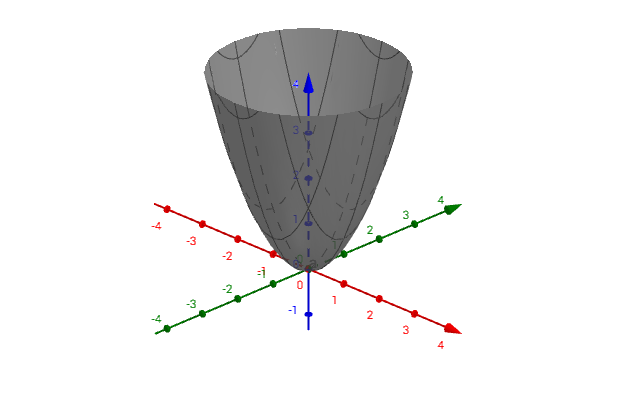
\includegraphics[width=.5\textwidth]{fig/UnderstandQuadraticForm_11.png}
\end{figure} 

半正定:
\begin{figure}[H]
    \centering
    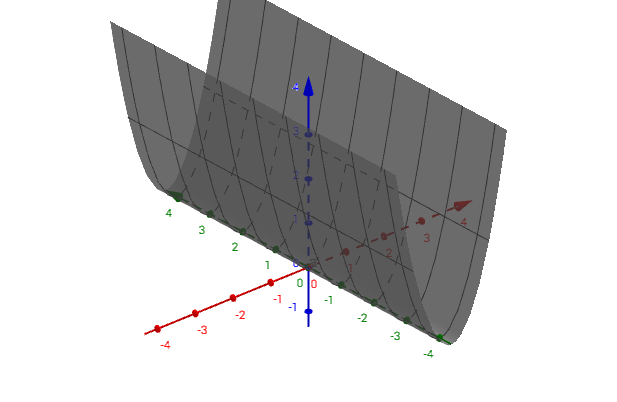
\includegraphics[width=.5\textwidth]{fig/UnderstandQuadraticForm_12.png}
\end{figure} 

不定:
\begin{figure}[H]
    \centering
    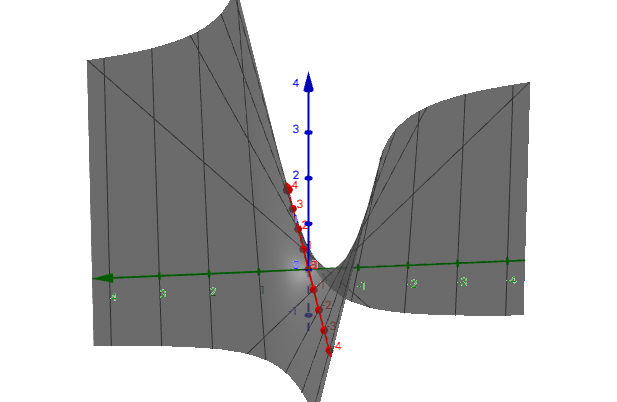
\includegraphics[width=.5\textwidth]{fig/UnderstandQuadraticForm_13.png}
\end{figure} 

既然二次型用矩阵来表示了,那么我们能否通过矩阵来判断是否正定呢?如果矩阵的特征值都大于0,则为正定矩阵。

\section{理解矩阵特征值和特征向量\cite{How_To_Understand_Eigen_Value_Vector}}
先给一个简短的回答,如果把矩阵看作是运动,对于运动而言,最重要的当然就是运动的速度和方向,那么(我后面会说明一下限制条件):
\begin{itemize}
    \item 特征值就是运动的速度
    \item 特征向量就是运动的方向
\end{itemize}

既然运动最重要的两方面都被描述了,特征值、特征向量自然可以称为运动(即矩阵)的特征。

注意,由于矩阵是数学概念,非常抽象,所以上面所谓的运动、运动的速度、运动的方向都是广义的,在现实不同的应用中有不同的指代。

\subsection{几何意义}
给定标准基$\vec{i},\vec{j}$和向量$\vec{v}$:
\begin{figure}[H]
    \centering
    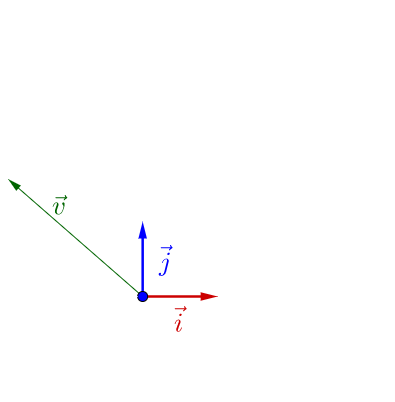
\includegraphics[width=.3\textwidth]{fig/UnderstandEigenValueVector_1.png}
\end{figure} 

随便左乘一个矩阵$A$,图像看上去没有什么特殊的:
\begin{figure}[H]
    \centering
    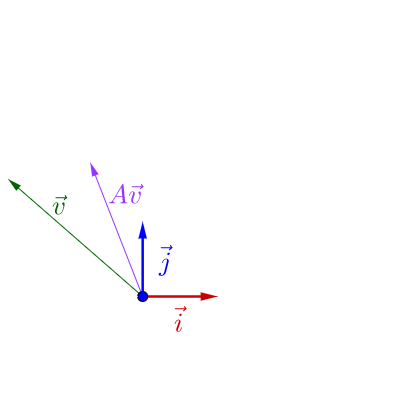
\includegraphics[width=.3\textwidth]{fig/UnderstandEigenValueVector_2.png}
\end{figure} 

但是调整下$\vec{v_{}}$的方向,图像看上去就有点特殊了:
\begin{figure}[H]
    \centering
    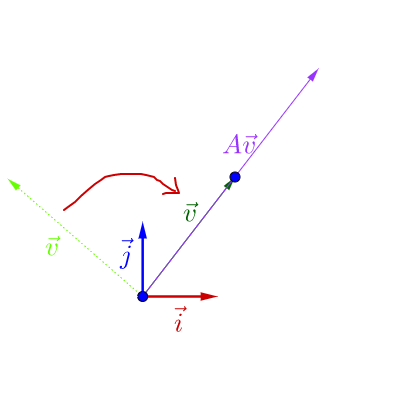
\includegraphics[width=.3\textwidth]{fig/UnderstandEigenValueVector_3.png}
\end{figure} 

可以观察到,调整后的$\vec{v_{}}$和$A\vec{v_{}}$在同一根直线上,只是$A\vec{v_{}}$的长度相对$\vec{v_{}}$的长度变长了。

此时,我们就称$\vec{v_{}}$是$A$的特征向量,而$A\vec{v_{}}$的长度是$\vec{v_{}}$的长度的$\lambda$倍,$\lambda$就是特征值。

从而,特征值与特征向量的定义式就是这样的:

\begin{figure}[H]
    \centering
    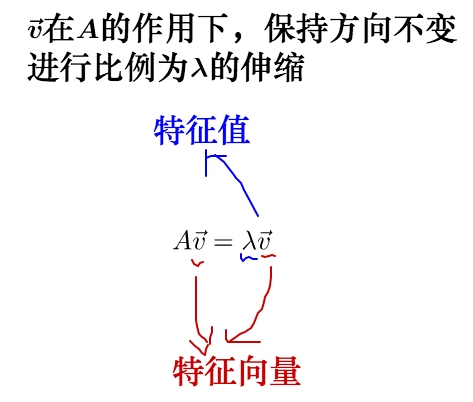
\includegraphics[width=.5\textwidth]{fig/UnderstandEigenValueVector_4.png}
\end{figure} 

其实之前的A不止一个特征向量,还有另一个特征向量:
\begin{figure}[H]
    \centering
    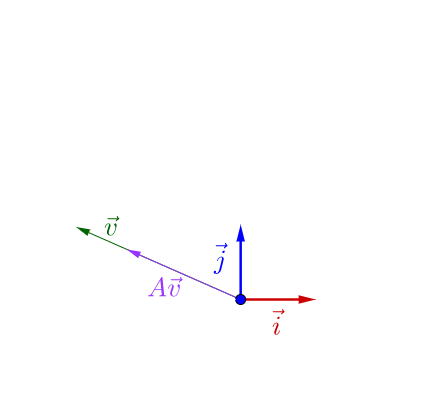
\includegraphics[width=.3\textwidth]{fig/UnderstandEigenValueVector_5.png}
\end{figure} 

容易从$A\vec{v_{}}$相对于$\vec{v_{}}$是变长了还是缩短看出,这两个特征向量对应的特征$\lambda$值,一个大于1,一个小于1。

从特征向量和特征值的定义式还可以看出,特征向量所在直线上的向量都是特征向量:
\begin{figure}[H]
    \centering
    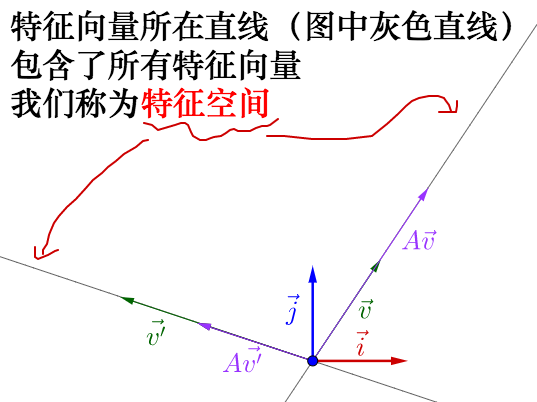
\includegraphics[width=.3\textwidth]{fig/UnderstandEigenValueVector_6.png}
\end{figure} 

\subsection{特征值、特征向量与运动的关系}
\subsubsection{矩阵的混合}
一般来说,矩阵我们可以看作某种运动,而二维向量可以看作平面上的一个点(或者说一个箭头)。对于点我们是可以观察的,但是运动我们是不能直接观察的。要观察矩阵所代表的运动,需要把它附加到向量上才观察的出来。

单独做一次矩阵的左乘(运动):
\begin{figure}[H]
    \centering
    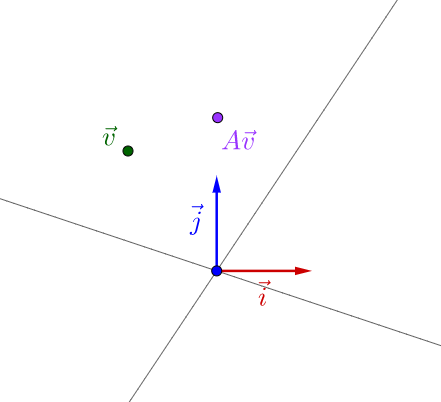
\includegraphics[width=.5\textwidth]{fig/UnderstandEigenValueVector_7.png}
\end{figure} 

似乎还看不出什么。但是如果我反复运用矩阵乘法的话:
\begin{figure}[H]
    \centering
    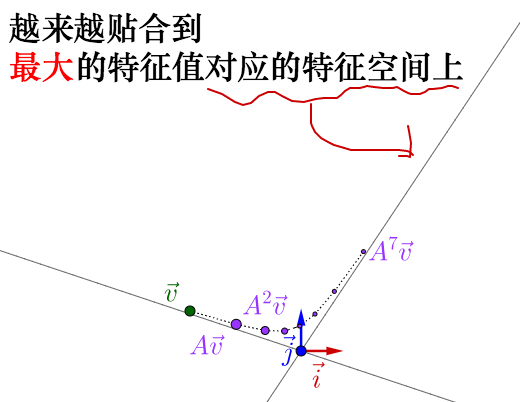
\includegraphics[width=.5\textwidth]{fig/UnderstandEigenValueVector_8.png}
\end{figure} 

也就是说,反复运用矩阵乘法,矩阵所代表的运动的最明显的特征,即速度最大的方向,就由最大特征值对应的特征向量展现了出来。

\subsection{特征值分解}
我们知道,对于矩阵$A$可以对角化的话,可以通过相似矩阵进行下面这样的特征值分解:
$$
A = P\Lambda P^{-1}
$$

其中$\Lambda$为对角阵,$P$的列向量是单位化的特征向量。

说的有点抽象,我们拿个具体的例子来讲:
\begin{figure}[H]
    \centering
    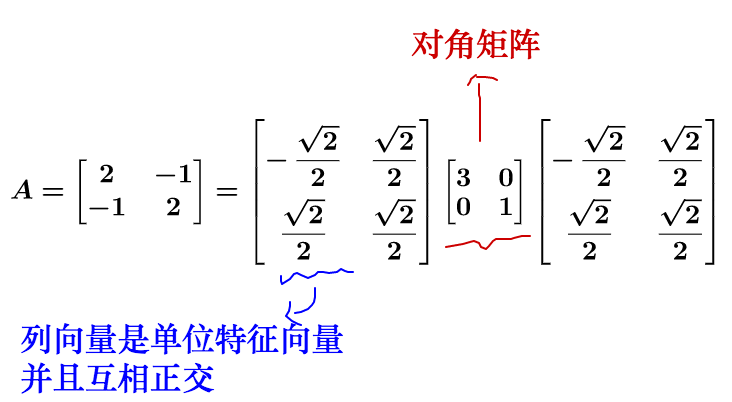
\includegraphics[width=.5\textwidth]{fig/UnderstandEigenValueVector_9.png}
\end{figure} 

对于方阵而言,矩阵不会进行纬度的升降,所以矩阵代表的运动实际上只有两种:旋转和拉伸,所以最后的运动结果就是这两种的合成。

我们再回头看下刚才的特征值分解,实际上把运动给分解开了:
\begin{figure}[H]
    \centering
    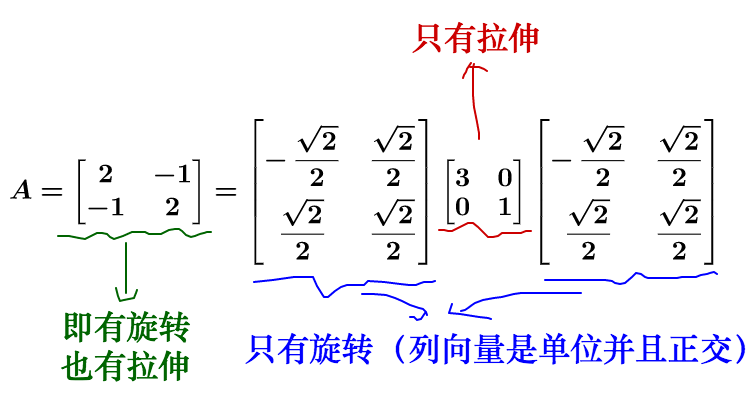
\includegraphics[width=.5\textwidth]{fig/UnderstandEigenValueVector_10.png}
\end{figure} 

%\printbibliography
\bibliography{../ref}
\bibliographystyle{IEEEtran}
\end{document}